\subsubsection{Definição}

Agora, a fim de definirmos as funções trigonométricas como funções
reais, considere a seguinte função, chamada de função de Euler: $E:
\reais \to \reais^2$ tal que $E(t)$ é o ponto $(x, y)$ do círculo
trigonométrico obtido após ``enrolarmos'', com uma corda de comprimento
$t$, o círculo trigonométrico iniciando no ponto $(1, 0)$ e tomando
como sentido positivo o sentido anti-horário. 
A construção é mostrada na Imagem~\ref{fig:ciclo-trigonometrico}.

\begin{figure}
\centering
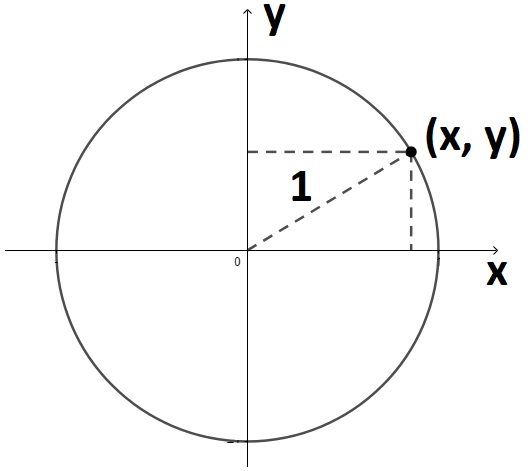
\includegraphics[scale=0.5]{\imgdirfromsection/circtrig.jpg}
\caption{Interpretação geométrica da função $E$}.
\label{fig:ciclo-trigonometrico}
\end{figure}

\begin{definition}
    As funções $\cos : \R \to \R$ e $\sen : \R \to \R$, chamadas
\textdef{função cosseno} e \textdef{função seno} respectivamente, são
definidas pondo-se, para cada $t \in \R$,
$$E(t) = \paren{\cos t , \sen t}.$$

Em outras palavras, $x= \cos t$ e $y = \sen t$ são, respectivamente,
a abcissa e a ordenada do ponto $E(t)$ da circunferência unitária.
\end{definition}

\begin{definition}
    Uma função $f: \R \to \R$ chama-se \textdef{periódica} quando existe $T
\in \R^\ast$ tal que $f(t + T) = f(t)$ para todo $t \in \reais$. Ao
menor número $T>0$ que faz a propriedade anterior ser satisfeita,
damos o nome de \textdef{período} da função $f$.
\end{definition}

\begin{remark}
    Como uma volta completa no círculo trigonométrico tem $2 \pi$ de
comprimento, é fácil ver que a função seno e cosseno são periódicas
de período $2\pi$.
\end{remark}

\begin{definition}
\label{def:funcao-par-impar}
    Uma função $f: \reais \to \reais$ é \textdef{par} quando se tem $f(-t) = f(t)$
para todo $t\in \reais$. Se for o caso de $f(-t) = - f(t)$ para todo $t
\in \reais$, dizemos que $f$ é \textdef{ímpar}.
\end{definition}

 \begin{proposition}
     A função seno é ímpar, e a função cosseno é par.
 \end{proposition}

 Segue imediatamente da definição das funções trigonométricas que a
relação fundamental $$ \sen^2 t + \cos^2 t = 1$$ vale para todo $t
\in \reais$.
Além disso, valem as seguintes igualdades para todo $t \in \reais$:
\begin{center}
\begin{tabular}{ c c }
    %\hline
    % after \\: \hline or \cline{col1-col2} \cline{col3-col4} ...
    $\cos \paren{t+ \pi} = -\cos t$, & $\sen \paren{t+ \pi} = -\sen t$, \\
    $\cos \paren{t+ \frac {\pi} 2} = -\sen t$, & $\sen \paren{t+ \frac {\pi} 2} = \cos t$, \\
    $\cos \paren{ \frac {\pi} 2 -t} = \sen t$, & $\sen \paren{ \frac {\pi} 2 -t} = \cos t$, \\
    $\cos \paren{ \pi -t} = -\cos t$, & $\sen \paren{ \pi -t} = \sen t$. \\
    %\hline
  \end{tabular}
\end{center}

\begin{onlineact}
    \khan{}https://pt.khanacademy.org/math/trigonometry/unit-circle-trig-func/trig-values-special-angles/e/trigonometric-functions-of-special-angles
    {Valores Trigonométricos de Ângulos Especiais}.
\end{onlineact}

\begin{onlineact}
    \khan{https://pt.khanacademy.org/math/trigonometry/unit-circle-trig-func/pythagorean-identity/e/circles-and-pythagorean-identities}
    {Use a Identidade Trigonométrica Fundamental}.
\end{onlineact}

\begin{onlineact}
    \khan{https://pt.khanacademy.org/math/trigonometry/trig-equations-and-identities/basic-sinusoidal-equations/e/solve-basic-sinusoidal-equations}
    {Resolva Equações Senoidais (Básico)}.
\end{onlineact}
